\documentclass{article}

% Language setting
% Replace `english' with e.g. `spanish' to change the document language
\usepackage[spanish]{babel}

\addto\captionsspanish{\renewcommand{\figurename}{Fig.}}

% Set page size and margins
% Replace `letterpaper' with `a4paper' for UK/EU standard size
\usepackage[letterpaper,top=2cm,bottom=2cm,left=3cm,right=3cm,marginparwidth=1.75cm]{geometry}

% Useful packages
\usepackage{amsmath}
\usepackage{graphicx}
\usepackage[colorlinks=true, allcolors=blue]{hyperref}

\title{Informe - Simulación de Sistemas - Grupo 2}
\author{
  Máximo Chiatellino \and
  Nombre Apellido \and
  Otro Nombre
}

\begin{document}
\maketitle

\begin{abstract}
Your abstract.
\end{abstract}

\section{Introducción}

Your introduction goes here! Simply start writing your document and use the Recompile button to view the updated PDF preview. Examples of commonly used commands and features are listed below, to help you get started.

Once you're familiar with the editor, you can find various project settings in the Overleaf menu, accessed via the button in the very top left of the editor. To view tutorials, user guides, and further documentation, please visit our \href{https://www.overleaf.com/learn}{help library}, or head to our plans page to \href{https://www.overleaf.com/user/subscription/plans}{choose your plan}.

\section{Modelo}

Se analiza un sistema de \(N\) partículas auto-propulsadas en un dominio cuadrado \([0,L]^2\) con condiciones de borde periódico (el plano se transforma en un toroide). Cada partícula avanza a módulo de velocidad constante \(v_0\) y está caracterizada por una orientación \(\theta_i(t)\). Estas partículas interactuan entre sí: cada partícula se alimenta de información con aquellas que se encuentran dentro de un disco de radio \(R_c\). Además, se adiciona otro elemento: el \textbf{ruido}, un valor aleatorio que perturba a las partículas alterando el ángulo con el que se trasladan.

\subsection{Escenario I: Standard Vicsek Model (SVM) \cite{vicsek1995}}
El SVM representa el mecanismo de \emph{alineamiento promedio con ruido angular}. En cada paso temporal todas las partículas actualizan su orientación de forma sincrónica según:
\begin{enumerate}
  \item \textbf{Alineación de la dirección de movimiento:} la nueva dirección de una partícula (\(\theta(t+1)\)) es el ángulo promedio de las direcciones de los vecinos (incluida la propia partícula) dentro de \(R_c\), \(\langle\theta(t)\rangle_r\). Operativamente, esto equivale a tomar la dirección del vector suma de las velocidades unitarias de las partículas vecinas.
  \item \textbf{Ruido angular:} a esa dirección se le agrega un ruido (\(\Delta \theta\)) elegido con probabilidad uniforme en el rango de amplitud \([-\eta/2, \eta/2]\), que modela incertidumbre en la orientación.
\end{enumerate}
Tras fijar la orientación (\(\theta(t+1)= \langle\theta(t)\rangle_r + \Delta \theta\)), cada partícula avanza una distancia \(v_0\Delta t\) en su nueva dirección (\(x_i(t+1) = x_i(t) + v_0\Delta t\)) . Conceptualmente: el acoplamiento local tiende a \emph{coherenciar} las direcciones, mientras que el ruido los \emph{dispersa}. Al aumentar \(\eta\) (o disminuir \(\rho\)), el sistema transita de un estado globalmente ordenado (\(\langle v_a\rangle>0\)) a uno desordenado (\(\langle v_a\rangle\approx 0\)).

\subsection{Escenario II: Flocking con interacciones tipo votante \cite{baglietto2018}}
Este escenario implementa un mecanismo \emph{imitativo} en lugar del promedio vectorial. En cada paso:
\begin{enumerate}
  \item \textbf{Imitación local:} cada partícula selecciona al azar un solo vecino dentro de \(r\) y \emph{copia} su orientación instantánea.
  \item \textbf{Fluctuación:} puede añadirse un ruido angular pequeño de amplitud \(\eta\) para evitar estados absorbentes perfectos.
\end{enumerate}

\section{Implementación}

Cada simulación recibe como input dos archivos: el primero, estático, una lista con la cantidad de partículas (\( N\)), el largo y ancho de la grilla (\( L\)) y los radios de cada una de las partículas (\( r_c\)). El segundo input consta la lista de posiciones iniciales (\(\mathbf x_0\)) de cada una de las partículas junto con el ángulo inicial (\( \theta_0\) [rad]).

El output generado es un archivo binario que detalla para cada timestep (\(t_i\)), la posición de cada partícula \(\mathbf x_i(t)\) así como su velocidad  \(\mathbf v_i(t)\) y el ángulo de la partícula (\( \theta_i\)).

\section{Simulaciones}

Para el análisis se contará con unidades adimensionales. Para las distancias se empleará "u" que representa la unidad de longitud de la simulación. Cada paso temporal discreto será denominado "step".

\subsection{Geometría}

El dominio de la simulación es una grilla de \(L\times L\) con condiciones de borde periódico, por lo que se comporta como un toroide.

\subsection{Parámetros y output}

Se listan a continuación los parámetros iniciales fijos de todas  las simulaciones:

\begin{itemize}
    \item La velocidad de las partículas se fija en \( v = 0.150 \) [u/step], encontrándose esta dentro del rango recomendado (Vicsek, 1995)
    \item Se simulan 2000 pasos para cada simulación. El estado inicial es  \( t_{min} = 0\) [step] mientras que el final es  \(t_{max} = 2000\) [step];
    \item Radio de interacción \(r_c\) = 1 [u].
    \item Radio de las partículas \(r\) = 0 [u].
\end{itemize}

\paragraph{Ruido a densidad fija:} Con \(\rho=2.5\) (combinaciones de \((N,L)\) más abajo), se grafica \(\eta\in[0,5]\) con \(\eta_i=0,2\times i\), \(i\in[0;25]\). Para cada \(\eta_i\) se ejecutan 5 réplicas independientes con posiciones (\(\mathbf x_0\)) y ángulos de las partículas (\( \theta_0\)) generados aleatoriamente para cada simulación.

\paragraph{Densidad a ruido fijo:} Con \(L=20\) y \(\eta=1\), se varía \(N_i=200\,i\), \(i \in [1,20]\), cubriendo \(\rho\in[0.5,10]\). También se corren 5 réplicas por condición con los mismos criterios.


\subsection{Observable}
El observable primario utilizado para determinar el orden colectivo se cuantifica con la \textbf{polarización} \(v_a\), el valor absoluto de la velocidad promedio normalizada.
\[
v_a(t) \;=\; \frac{1}{N v_0}\,\Big|\sum_{i=1}^N \mathbf v_i(t)\Big|\in[0,1],
\]
el \(v_a\) distingue el régimen desordenado (\(\approx 0\)) del polar (\(\approx 1\)).

Se analiza cómo varía la polarización en función de la densidad y del ruido para cada uno de los dos modelos considerados.

\subsubsection{Polarización y ruido}
Primero, se grafica el \(t\) vs \(v_a(t)\) para \(\eta \in [0;5]\) dado que se busca observar el comportamiento de \( \eta \) vs.\ \( v_a(t) \) manteniendo la densidad constante para distintas combinaciones de \( L \) y \( N \).  Para cada una de las simulaciones con un determinado \(\eta_i\) se realizan 5 variantes. Para cada \(\eta_i\), se toman los últimos 400 pasos (el último 20\%) de \(v_a(t)\) de cada una de las 5 iteraciones (en total, \(5\times 400=2000\) valores) para estudiar el comportamiento del observable. Con ese conjunto agregado se calcula la media \(\mu_\eta\) y el desvío estándar \(\sigma_\eta\) donde \(v_{a_i}(t)\) denota la polarización en el paso \(t\) de la iteración \(i\):

\[
\mu_{\eta} \;=\; \frac{1}{2000}\,\sum_{i=0}^{4}\,\sum_{t=1601}^{2000} v_{a_i}(t)
\]

\[
\sigma_{\eta} \;=\; \sqrt{\frac{1}{2000}\,\sum_{i=0}^{4}\,\sum_{t=1601}^{2000}\Bigl(v_{a_i}(t)-\mu_{\eta}\Bigr)^2}
\]


Se analiza el comportamiento del sistema en los siguientes casos, para encontrar posibles variaciones en los resultados de acuerdo al \(N\) y \(L\) utilizados para calcular la densidad:
\begin{itemize}
    \item \(N=1000\) y \(L=20\),
    \item \(N=500\) y \(L=14,142\)
    \item \(N=250\) y \(L=10\)
\end{itemize}

\subsubsection{Polarización y densidad}
A continuación, se conducen las simulaciones correspondientes para analizar   \(t\) vs \(v_a(t)\) para una serie  \(\rho\in [0;10]\). En este caso se mantiene el ruido como parámetro fijo, de modo que el sistema no converja a un orden total.
Al igual que lo explicado para el análisis del ruido, se realizan 5 ejecuciones de la simulación para cada \(N_i\) y se elige el último 20\% de los valores de \(v_a(t)\) para el análisis.

\section{Resultados}
\subsection{Polarización y Ruido}
\subsubsection{Modelo Estándar de Vicsek}

\begin{figure}
    \centering
    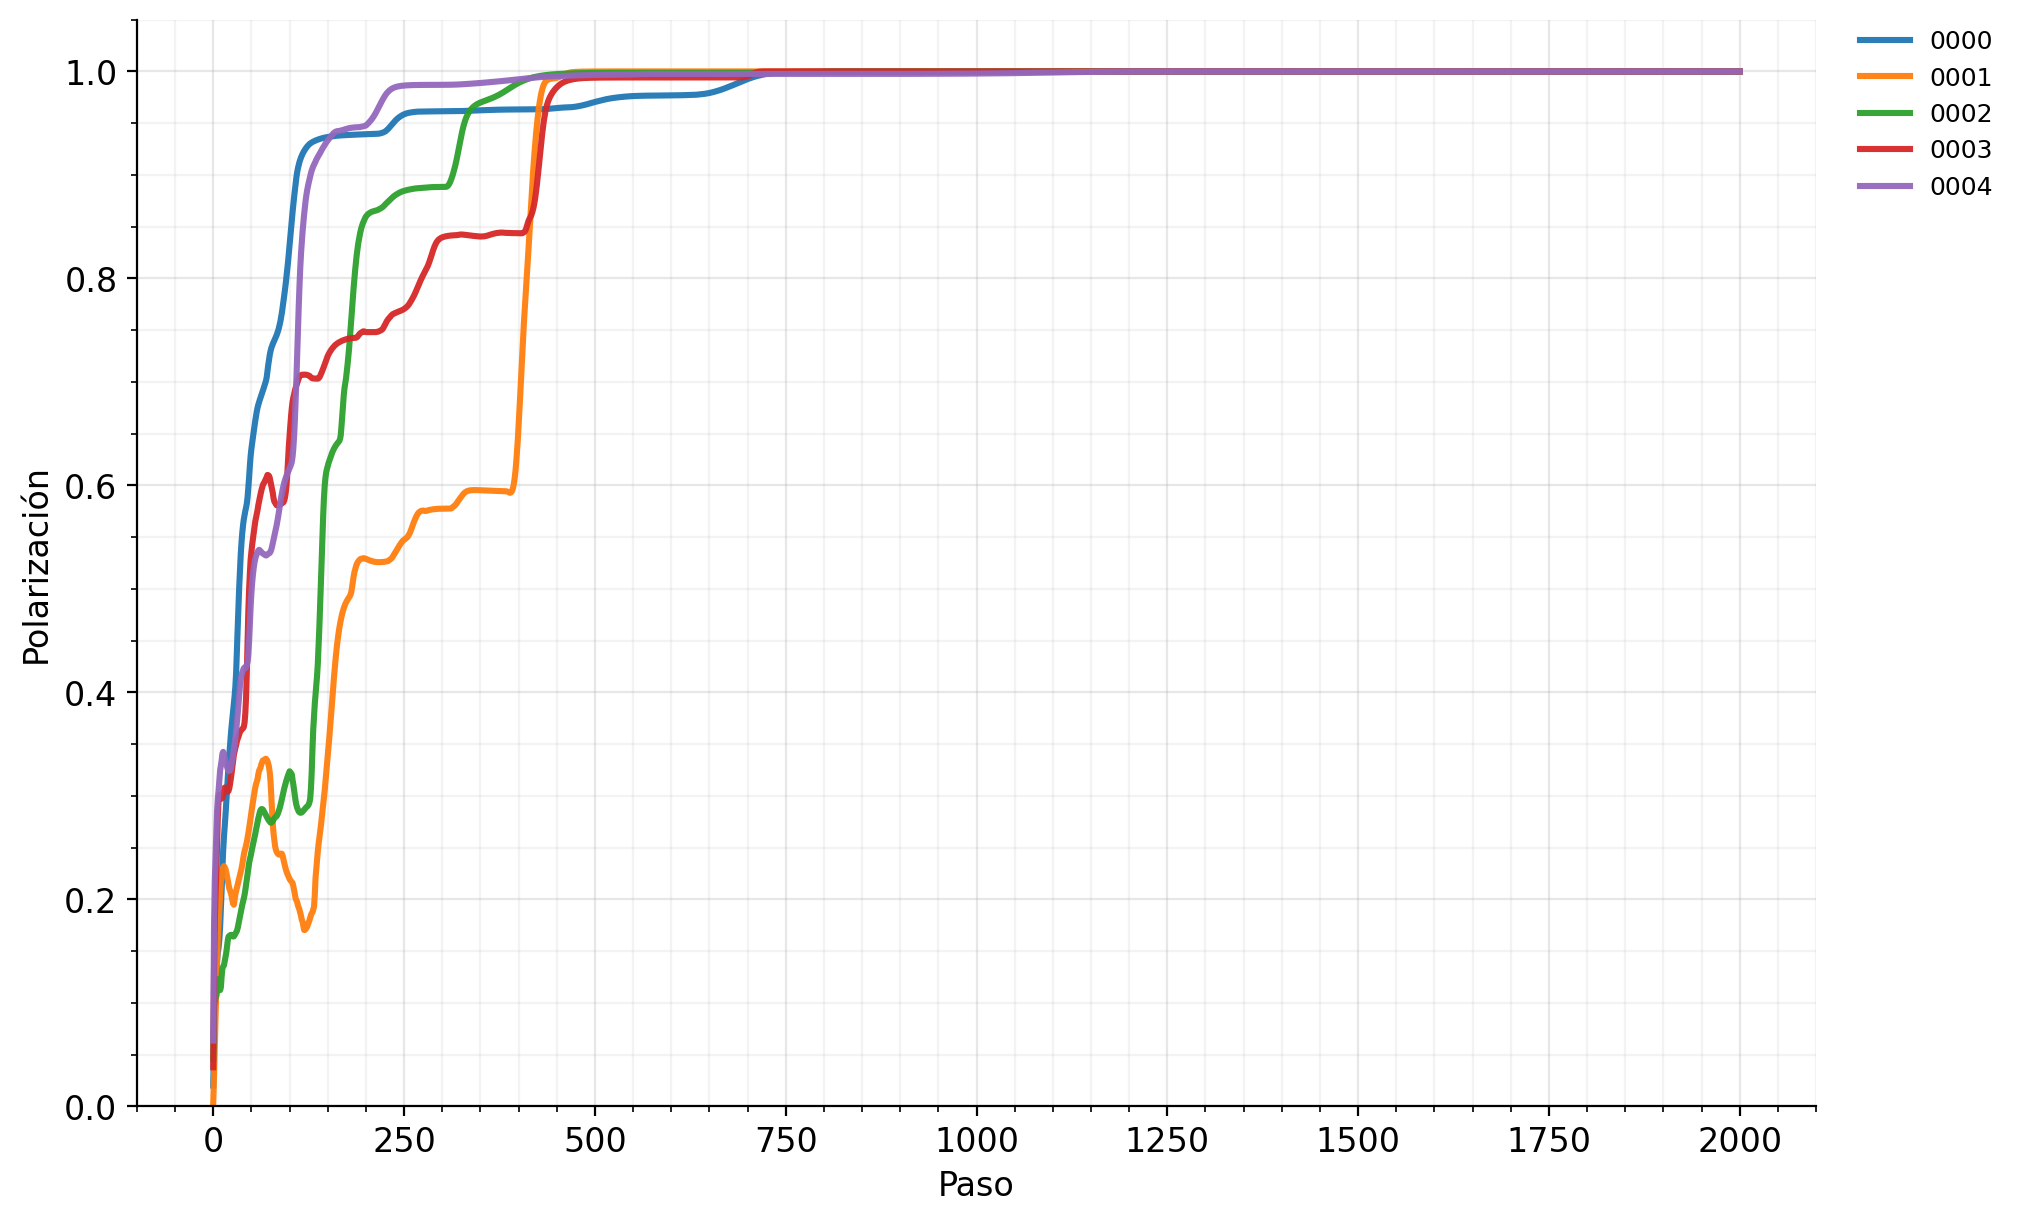
\includegraphics[width=1\linewidth]{noise_0_SVM.png}
    \caption{Con \(\eta = 0)\)}
    \label{Fig. 1:}
\end{figure}
\subsubsection{Modelo de los Votantes }


\section{Conclusiones}

Simply use the section and subsection commands, as in this example document! With Overleaf, all the formatting and numbering is handled automatically according to the template you've chosen. If you're using the Visual Editor, you can also create new section and subsections via the buttons in the editor toolbar.

\subsection{How to include Figures}

First you have to upload the image file from your computer using the upload link in the file-tree menu. Then use the includegraphics command to include it in your document. Use the figure environment and the caption command to add a number and a caption to your figure. See the code for Figure \ref{fig:frog} in this section for an example.

Note that your figure will automatically be placed in the most appropriate place for it, given the surrounding text and taking into account other figures or tables that may be close by. You can find out more about adding images to your documents in this help article on \href{https://www.overleaf.com/learn/how-to/Including_images_on_Overleaf}{including images on Overleaf}.



\subsection{How to add Comments and Track Changes}

Comments can be added to your project by highlighting some text and clicking ``Add comment'' in the top right of the editor pane. To view existing comments, click on the Review menu in the toolbar above. To reply to a comment, click on the Reply button in the lower right corner of the comment. You can close the Review pane by clicking its name on the toolbar when you're done reviewing for the time being.

Track changes are available on all our \href{https://www.overleaf.com/user/subscription/plans}{premium plans}, and can be toggled on or off using the option at the top of the Review pane. Track changes allow you to keep track of every change made to the document, along with the person making the change.

\subsection{How to add Lists}

You can make lists with automatic numbering \dots

\begin{enumerate}
\item Like this,
\item and like this.
\end{enumerate}
\dots or bullet points \dots
\begin{itemize}
\item Like this,
\item and like this.
\end{itemize}

\subsection{How to write Mathematics}

\LaTeX{} is great at typesetting mathematics. Let $X_1, X_2, \ldots, X_n$ be a sequence of independent and identically distributed random variables with $\text{E}[X_i] = \mu$ and $\text{Var}[X_i] = \sigma^2 < \infty$, and let
\[S_n = \frac{X_1 + X_2 + \cdots + X_n}{n}
      = \frac{1}{n}\sum_{i}^{n} X_i\]
denote their mean. Then as $n$ approaches infinity, the random variables $\sqrt{n}(S_n - \mu)$ converge in distribution to a normal $\mathcal{N}(0, \sigma^2)$.


\subsection{How to change the margins and paper size}

Usually the template you're using will have the page margins and paper size set correctly for that use-case. For example, if you're using a journal article template provided by the journal publisher, that template will be formatted according to their requirements. In these cases, it's best not to alter the margins directly.

If however you're using a more general template, such as this one, and would like to alter the margins, a common way to do so is via the geometry package. You can find the geometry package loaded in the preamble at the top of this example file, and if you'd like to learn more about how to adjust the settings, please visit this help article on \href{https://www.overleaf.com/learn/latex/page_size_and_margins}{page size and margins}.

\subsection{How to change the document language and spell check settings}

Overleaf supports many different languages, including multiple different languages within one document.

To configure the document language, simply edit the option provided to the babel package in the preamble at the top of this example project. To learn more about the different options, please visit this help article on \href{https://www.overleaf.com/learn/latex/International_language_support}{international language support}.

To change the spell check language, simply open the Overleaf menu at the top left of the editor window, scroll down to the spell check setting, and adjust accordingly.

\subsection{How to add Citations and a References List}

You can simply upload a \verb|.bib| file containing your BibTeX entries, created with a tool such as JabRef. You can then cite entries from it, like this: \cite{greenwade93}. Just remember to specify a bibliography style, as well as the filename of the \verb|.bib|. You can find a \href{https://www.overleaf.com/help/97-how-to-include-a-bibliography-using-bibtex}{video tutorial here} to learn more about BibTeX.

If you have an \href{https://www.overleaf.com/user/subscription/plans}{upgraded account}, you can also import your Mendeley or Zotero library directly as a \verb|.bib| file, via the upload menu in the file-tree.

\subsection{Good luck!}

We hope you find Overleaf useful, and do take a look at our \href{https://www.overleaf.com/learn}{help library} for more tutorials and user guides! Please also let us know if you have any feedback using the \textbf{Contact us} link at the bottom of the Overleaf menu --- or use the contact form at \url{https://www.overleaf.com/contact}.

\bibliographystyle{alpha}
\bibliography{sample}

\end{document}